\documentclass[aps,reprint]{revtex4-1}
% Engine-specific settings
% Detect pdftex/xetex/luatex, and load appropriate font packages.
% This is inspired by the approach in the iftex package.
% pdftex:
\ifx\pdfmatch\undefined
\else
    \usepackage[T1]{fontenc}
    \usepackage[utf8]{inputenc}
\fi
% xetex:
\ifx\XeTeXinterchartoks\undefined
\else
    \usepackage{fontspec}
    \defaultfontfeatures{Ligatures=TeX}
\fi
% luatex:
\ifx\directlua\undefined
\else
    \usepackage{fontspec}
\fi
% End engine-specific settings
\usepackage[english]{babel}
\usepackage{csquotes}
% \usepackage[backend=biber, sortcites]{biblatex}
\usepackage{url}
\usepackage{textcomp}
\usepackage[usenames,dvipsnames,svgnames, table]{xcolor}
\usepackage[font={scriptsize}]{caption}
\usepackage{amsmath} \usepackage{amsthm} \usepackage{amsfonts}
\usepackage{amssymb}
\usepackage{enumerate}
\usepackage{tikz} \usepackage{float}
\usepackage[procnames]{listings}
\usepackage{pstool} \usepackage{pgfplots}
\usepackage{wrapfig} \usepackage{graphicx} \usepackage{epstopdf}
\usepackage{afterpage}
\usepackage{physics}
\usepackage{multirow}
\usepackage{gensymb}
\usepackage{algorithm}
\usepackage{microtype}
\usepackage[noend]{algpseudocode}
\usepackage{xcolor,colortbl}
\usepackage{microtype}
\usepackage{geometry}
\usepackage{hyperref}
\usepackage{graphicx}
\usepackage{caption}
\usepackage{subcaption}
\usepackage{lipsum}
% \usepackage{pythontex}
% \usepackage{authblk}
\usepackage{nth}
\usepackage{siunitx}
% \usepackage[toc,page]{appendix}
\floatstyle{plaintop}
\restylefloat{table}

% Custom commands
\newcommand{\unit}[1]{\:\mathrm{#1}}
\newcommand{\noref}[1]{\hyperref[#1]{\ref*{#1}}}
\newcommand{\nonref}[1]{\hyperref[]{\ref*{#1}}}
\newcommand\blankpage{%
  \null
  \thispagestyle{empty}%
  \addtocounter{page}{-1}%
  \newpage}

% Default fixed font does not support bold face
\DeclareFixedFont{\ttb}{T1}{txtt}{bx}{n}{7} % for bold
\DeclareFixedFont{\ttm}{T1}{txtt}{m}{n}{7}  % for normal

\newcommand\numberthis{\addtocounter{equation}{1}\tag{\theequation}}
\DeclareCaptionFont{white}{\color{white}}
\DeclareCaptionFormat{listing}{\colorbox{gray}{\parbox{\columnwidth}{#1#2#3}}}
\pgfplotsset{compat=1.14} %TODO: Setting this removed several error messages, should it be here!?


% Biber for references
% \bibliographystyle{aipauth4-1}

\begin{document}
\sisetup{detect-all}
\title{Simulation of the solar system with numerical methods}
\author{Erlend Lima}
\author{Frederik J. Mellbye}
\affiliation{University of Oslo, Oslo, Norway \\ Source code available at: \url{https://github.com/Caronthir/FYS3150/tree/master/Project3}}
\date{\today}

\begin{abstract}
Two numerical algorithms are used to solve systems of coupled ODE's by simulating a n-body problem, our solar system.
The algorithms used are the Forward Euler and Velocity-Verlet algorithms. With only X extra floating point operations per
iteration of the algorithm, the Verlet method is shown to completely outperform the Euler scheme in terms of numerical accuracy and stability,
with a small cost in execution speed. By investigating the solutions for different step sizes, $10^5$ time steps per year resulted in
solutions with an acceptable compromise between numerical precision and speed. The perihelion precession of Mercury (which
was predicted by general relativity) was also reproduced by the numerical implementation.
\end{abstract}
\maketitle
\tableofcontents
\makeatletter
\let\toc@pre\relax
\let\toc@post\relax
\makeatother

\newpage

\section{Introduction}
\label{sec:introduction}
The n-body problem consists of predicting the individual motions of a group of objects
interacting with each other gravitationally. The motivation for finding solutions
to this problem comes from the desire to understand the relative motion of the
objects in the solar system. The methods used to solve these types of problems are also applicable in
similar problems in statistical and molecular dynamics.

For the simple case of two celestial bodies it is trivial to solve the time
development of the system analytically. When more objects are added however,
analytical solutions are hard to come by, and numerical methods are required to find
approximated solutions.

In this paper, the equations of motion are written as a coupled set of first-order linear equations, and
the classic forward Euler and Velocity Verlet algorithms are employed to simulate the solar system,
and their accuracies, conservation properties and computation times are compared. The theoretical
model for the forces in our solar system (Newtonian gravity) is derived, and the numerical implementations
are used to solve the time development of the planets in the solar system. Several analytical results are reproduced by the program, such as conservation of energy and angular momentum, escape velocities and the perihelion precession of Mercury.
\section{Theory}
\label{sec:theory}
For planetary motion, the only force present is gravity. Newton's law of gravitation
states that any two objects in the universe attract each other by a force given
by
\begin{align}
  F_G = \frac{G m_1 m_2}{r^2}
\end{align}
where $m_1$ and $m_2$ are the masses of the objects, $G$ is the
gravitational constant and $r$ is the distance between the objects. In the
case examined in this paper, it is assumed that the solar mass is much larger
than the planet masses ($M_\odot \gg M_\text{planet}$), and the solar
movement is therefore ignored. Then, for a planet orbiting the sun, the
planet position as a function of time is described by Newton's second law:
\begin{align*}
  \dv[2]{\mathbf{x}}{t} = \frac{\mathbf{F}_G}{M}
\end{align*}
where $M$ is the planet mass. This is equivalent to one ODE (ordinary differential
equation) for each direction component, i.e. three separate equations in the
three-dimensional case.

For the numerical methods the above second order vector ODE is more convenient to
work with when written as a set of two coupled first order equations. These
are given by
\begin{align}
  \begin{split}
  \label{eq:coupledequations}
  \dv{x}{t} &= v(x,t) \\
  \dv{v}{t} &= \frac{F(x,t)}{M} = a(x,t)
  \end{split}
\end{align}
These equations are solved for three dimensions. Note that the gravitational force,
and hence the acceleration, depends on the distance between the celestial bodies.
This results in six coupled, first-order, linear differential equations.

The algorithms used are both based on Taylor expansions, the forward Euler
scheme approximates position and velocity to first order, while the Verlet
method combines a second order approximation with the fact that the acceleration
is only position dependent. In the following the algorithims are stated.

\subsection{Forward Euler}
The Euler method (forward Euler) is the most basic numerical method to solve
ODEs. This widely known algorithm applied to ~\ref{eq:coupledequations} is given by
\begin{align*}
  \begin{split}
  v_{i+1} = v_{i} + a_{i}\Delta{t} \\
  x_{i+1} = x_{i} + v_{i}\Delta{t}
\end{split}
\end{align*}
These equations are derived by simply Taylor expanding the position and velocity
and omitting the error terms.
\subsection{Velocity Verlet}
The velocity Verlet method is based on Taylor-expanding the position and velocity
to second order, and specialized for cases where the acceleration is only
dependent on position. The algorithm (see ~\ref{sec:velocityverlet} for details)
applied to the problem examined in this paper is given by the following equations:
\begin{align}
  \begin{split}
    x_{i+1} &= x_i + v_i + \frac{\Delta{t}^2}{2} a_i \\
    v_{i+1} &= v_i + \frac{\Delta{t}}{2}(a_{i+1} + a_{i})
  \end{split}
\end{align}
Note that this algorithm assumes $a_{i+1}$ is only dependent on position $x_{i+1}$
and not velocity $v_{i+1}$. This is because the acceleration in the next step
is required to calculate the velocity in the next step. Because $a_{i+1} = a(x_{i+1})$,
the position in the next step is computed prior to the velocity. This algorithm
therefore is suited to solve for planetary motion, because gravity is only
position dependent and the only force that acts within the system.

\subsection{Initial conditions}
To find a unique solution to the set of coupled equations a set of initial conditions needs
to be specified. For the set of three coupled second order equations solved in this project,
initial positions and velocities are required for each spatial dimension. That is,
\begin{align*}
 \mathbf{x_0}(t = 0) \text{ and } \mathbf{v_0}(t = 0)
\end{align*}
are required for the sun and all planets and moons that are included in the simulation.

\subsection{Conservation laws for the system}
Because no external forces act on the system, total energy and angular momentum should
be conserved over time. Expressions for these quantities are shown separately.
\subsubsection{Energy}
The total energy of the system should be conserved. The kinetic energy of an object with
mass $m$ and velocity $v$ is given by
\begin{align*}
 E_k = \frac{1}{2}m v^2
\end{align*}
The expression for the gravitational potential energy of a massive object can be found by
integrating the gravitational force from the distance between the objects to some reference
distance, which is set to $r = \infty$ (i.e. using the definition of potential energy and the law
of gravitation). This yields
\begin{align*}
 E_p = -\int_\infty^r F_G \text{d} r = -\frac{GmM}{r}
\end{align*}
as the potential energy of an object (mass $m$) with respect to some object (mass $M$),
separated by a distance $r$.
\subsubsection{Angular momentum}
Yolo
\subsection{Escape velocity}
The escape velocity is the minimum speed needed for an object to escape from the
gravitational influence of an object with mass. One way to derive this velocity
is by energy conservation. The case with the Earth-Sun system
is examined, where at the initial state, Earth (with mass $M_E$) is at a
distance $r$ from the Sun (mass $M_\odot$). The
initial speed of the planet is the escape velocity $\mathbf{v_e}$, and at the
final state it will have moved infinitely far away ($r = \infty$) and the speed
will tend to zero. By conservation of energy
\begin{align*}
  (K + U)_0 &= (K + U)_1 \\
  \frac{1}{2} M_E \mathbf{v_e}^2 &= \frac{GM_E M_\odot}{r}
\end{align*}
which yields the size of the escape velocity
\begin{align}
  v_e = |\mathbf{v_e}| = \sqrt{\frac{2GM_\odot}{r}}
\end{align}
From the equations it is clear that the direction of the escape velocity is
arbitrary, because only energies need to be considered to arrive at the above
expression.

\subsection{Perihelion precession of Mercury}
In Newtonian physics, any object that orbits a massive star or planet will have a constant elliptical orbit with
the spherical mass approximately at focus. In the solar system, the closest point to the Sun of an orbit is called
the perihelion. Multiple effects in the solar system cause the elliptical orbits to rotate, in the sense that the perihelia
precesses around the sun. The most significant effect comes from the gravitational forces from the other bodies in
the solar system. For Mercury, the Newtonian based-explanations were insufficient in predicting the precession, and
this error was corrected when Einstein showed that results from general relativity closely agrees with the observed
perihelion precession. To correct for general relativity spacetime shift, the gravitational force can be modified to
\begin{align}
\label{eq:mercuryprecession}
\mathbf{F_G} = \frac{G M_\odot M_\text{Mercury}}{r^3}\left[1 + \frac{3l^2}{r^2c^2} \right] \hat{\mathbf{r}}
\end{align}
where $l = |\mathbf{l}|$ is the norm of the angular momentum per mass of Mercury, $c$ is the speed of light and
$\mathbf{r}$ is the relative position of Mercury with respect to the Sun.
\section{Method}
\label{sec:method}
\subsection{Choice of units}
For the Solar System it is convenient to use units that scale lengths, time and
masses to orders of magnitude that are easier to work with. The distances are
therefore in astronomical units (AU), which is defined to roughly the mean
distance between the Earth and the Sun. By the same token, time is measured in
years (yr) and masses are in solar masses $M_\odot$.

Examining Newton's law for Earth in the Earth-Sun system under the assumption
that the orbit is circular shows that
\begin{align*}
  \frac{GmM_\odot}{r^2} = m \frac{v^2}{r}
\end{align*}
where $m$ is Earth's mass and $r$ is the distance between the objects. In the
units chosen, $r = 1$ AU and the orbital velocity is given by the orbital distance
travelled per year $v = 2\pi \text{AU}/1 \text{yr}$. Then the gravitational
constant is given by
\begin{align}
  G = 4\pi^2 \text{AU}^3 \text{yr}^{-2} M_\odot^{-1}
\end{align}
\subsection{Initial values}
The initial values of the solar system bodies are fetched from the NASA HORIZONS
Web-Interface, see \cite{nasa}.
\subsection{Models}
In this project, four separate situations are tested. This makes it possible to test the versatility of the
algorithms in different circumstances, and to investigate multiple special situations.
\subsubsection{Earth-Sun system - Comparison of Forward Euler and Velocity-Verlet}
\label{seq:earthsunmethod}
For the simple case of the Earth-Sun system, the positions of the Sun and Earth are
forwarded for a year with both algorithms. The Sun is placed at the origin with
no initial velocity, and for simplicity Earth is given an initial position 1 AU
away from the Sun in the x-direction. It is given an initial velocity $v = 2\pi$ AU/yr
in the y-direction, which analytically should lead to a perfect circular motion
if the Sun is kept stationary. The simulation is done with $N = 1000$ time steps.
\subsubsection{Three-body problem}
The Earth-Sun system is expanded to include the most massive planet in the Solar System, Jupiter.
\subsubsection{Full Solar System simulation}
The simulation is here fully extended to include every planet (also Pluto, although Pluto is not considered a planet any more :( ).
\subsubsection{The perihelion precession of Mercury}
The gravitational force is modified to include general relativistic effects, and
the system is simulated with only the Sun and Mercury. The other planets are removed,
because only the relativistic effect on the perihelion precession is investigated.
To ensure that the time resolution in the simulation was sufficient, bla bla bla
was done.
\section{Results}
\label{sec:results}
\subsection{Earth-Sun system - Comparison of Euler and Verlet methods}
\begin{figure}[H]
  \centering
  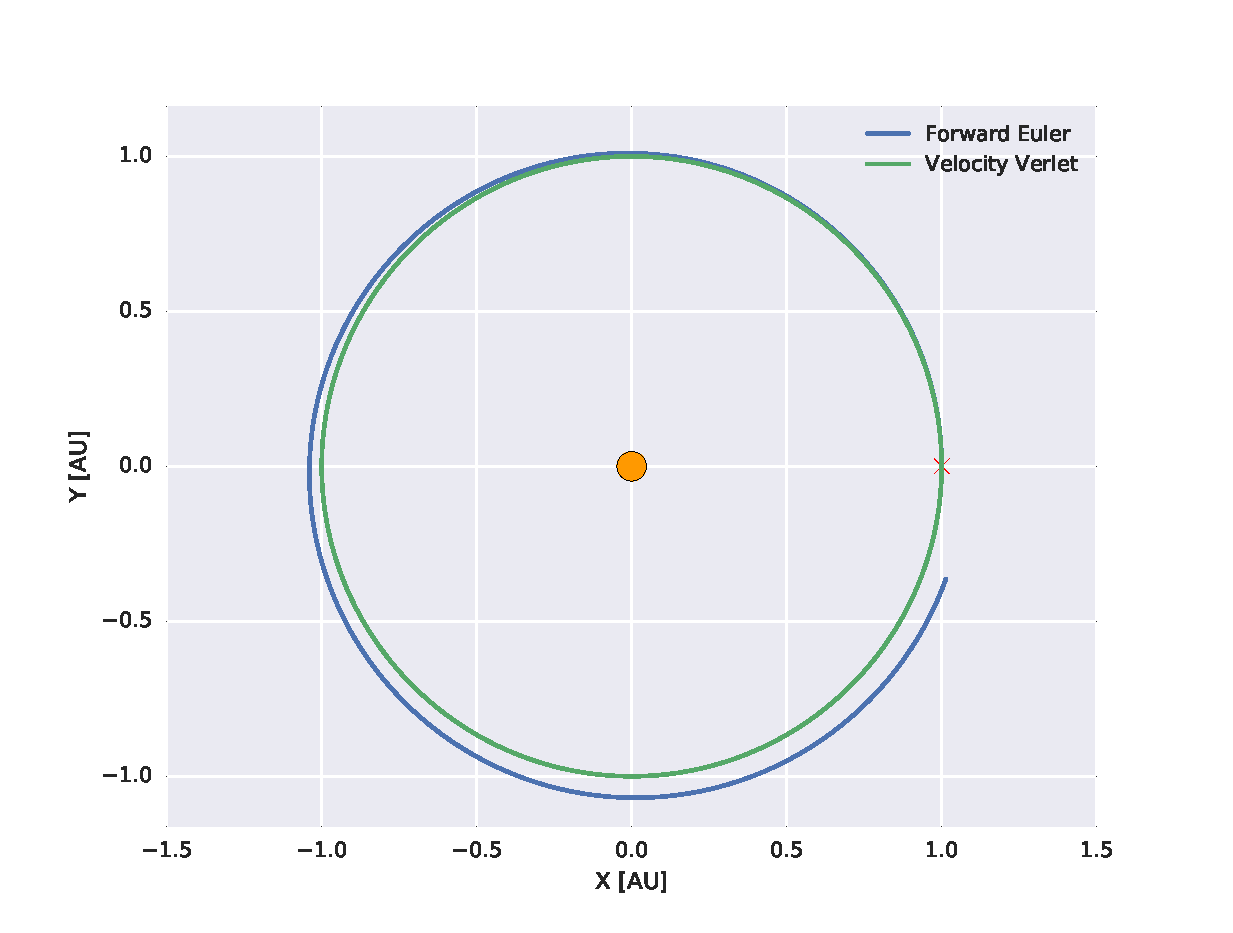
\includegraphics[width=\columnwidth]{figures/eulerverlet.eps}
  \caption{Position of the Earth forwarded for a year with the Euler and Verlet
  schemes. The initial position is marked with a red cross.}
  \label{fig:earthsunorbits}
\end{figure}
\subsection{Three-body problem}
\subsection{Full solar system simulation}
\subsection{The perihelion precession of Mercury}

\section{Discussion}
\label{sec:discussion}
Discussion of the results!
\section{Conclusion}
\label{sec:conclusion}
Concluding it all with a conclusion.
\bibliography{references}
\blankpage
\appendix
\section{Derivation of velocity Verlet algorithm}
\label{sec:velocityverlet}
The Velocity Verlet method is derived for one dimension ($x$), but is easily
generalized for three dimensions by simply repeating the procedure with $y$
or $z$ instead of $x$. The derivation can also be generalized to three dimensions
simply by considering $x$ as a vector $\mathbf{x} = (x, y, z)$.
The position and time is discretized to $n$ integration points so that
\begin{align*}
  x(t) &\rightarrow x(t_i) &&= x_i \\
  t &\rightarrow t_i &&= t_0 + i\Delta{t}
\end{align*}
where $\Delta{t} = \frac{t_\text{final} - t_0}{n-1}$ the time step size. The velocity
is similarly discretized to each time point so that $v(t) \rightarrow v_i$.
Taylor expanding the position and velocity yields
\begin{align*}
  x_{i+1} &= x_i + \Delta{t} x'_i + \frac{\Delta{t}^2}{2} x''_i + O(\Delta{t}^3) \\
  v_{i+1} &= v_i + \Delta{t} v'_i + \frac{\Delta{t}^2}{2} v''_i + O(\Delta{t}^3)
\end{align*}
The second derivative of the velocity is approximated using Euler's method, so
\begin{align*}
  \Delta{t} v''_i = v'_{i+1} - v'_{i} = a_{i+1} - a_{i}
\end{align*}
where $a_i$ is the acceleration at $t = t_i$. With this approximation for the
velocity second derivative, the Taylor expansions are given by
\begin{align*}
  v_{i+1} &= v_i + \Delta{t} a_i + \frac{\Delta{t}}{2} (a_{i+1} - a_i) + O(\Delta{t}^3) \\
          &= v_i + \frac{\Delta{t}}{2} (a_{i+1} + a_{i}) + O(\Delta{t}^3)
\end{align*}
For the numerical algorithm the error terms are omitted and the resulting
algorithm is
\begin{align}
  \begin{split}
    x_{i+1} &= x_i + v_i + \frac{\Delta{t}^2}{2} a_i \\
    v_{i+1} &= v_i + \frac{\Delta{t}}{2}(a_{i+1} + a_{i})
  \end{split}
\end{align}
\blankpage
\end{document}

% Local Variables:
% TeX-engine: luatex
% End:
